\begin{figure*}
  \centering
  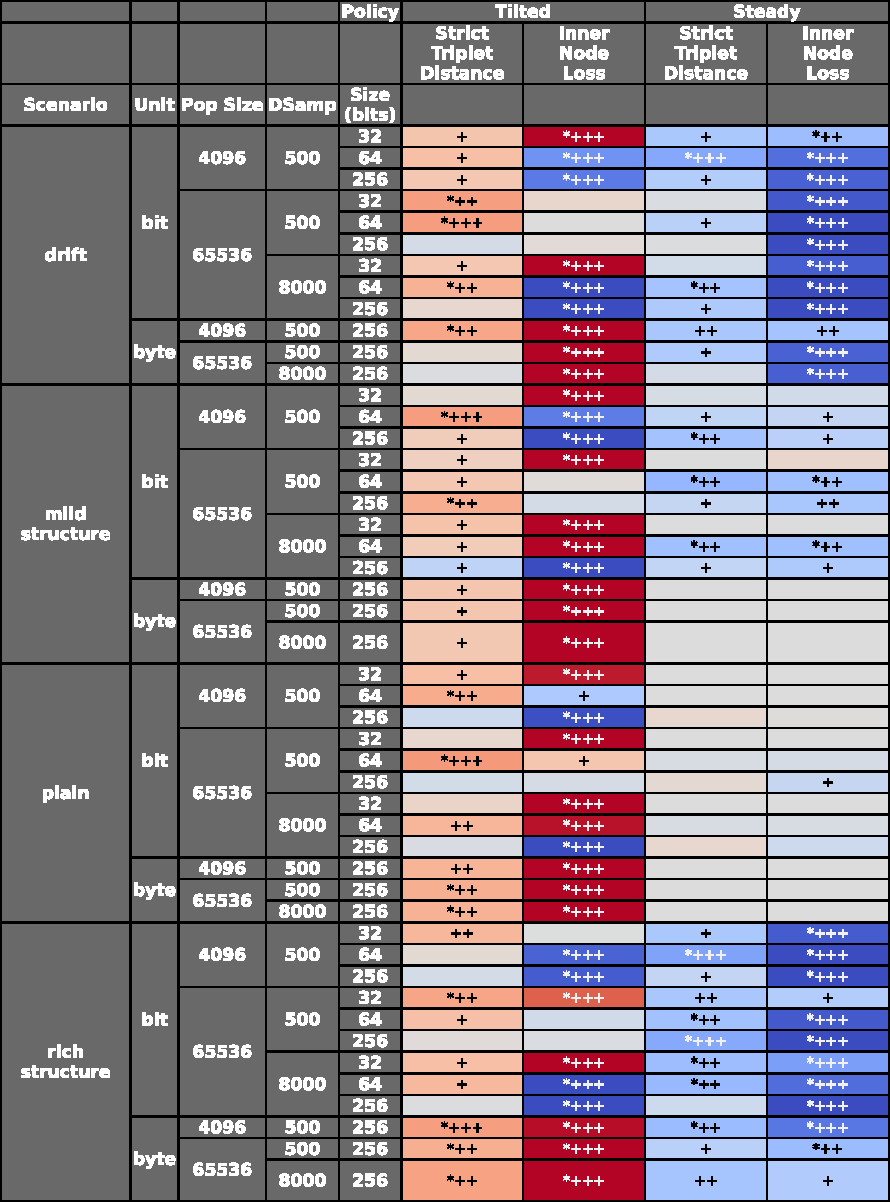
\includegraphics[width=\textwidth]{binder/binder/surf-vs-col/outplots/surf-vs-col-table}
  \caption{%
   \textbf{Comparison of reconstruction accuracies from column- and surface-based annotations.}
    Color coding represents non-parametric difference between accuracy measures, with red indicating superior surface performance and blue indicating superior column performance.
    Left column shows tilted retention policies, and right column shows steady retention policies.
    For heatmap charts, +'s indicate small, medium, and large effect sizes using the Cliff's delta statistic and *'s indicate statistical significance at $\alpha = 0.05$ via Mann-Whitney U test.
  }
  \label{fig:col-vs-surf}
\end{figure*}
